\chapter{How to model a system}\label{How to model a system}
\begin{aquote}{The Chemical Basis of Morphogenesis. A. Turing 1952.}
\textit{This model will be a simplification and an idealization, and consequently a falsification. It is to be hoped that the features retained for discussion are those of greatest importance in the present state of knowledge.}
\end{aquote}
\begin{aquote}{Empirical Model-Building and Response Surfaces. G. Box \& N. Draper 1987.}
\textit{All models are wrong, but some are useful.}
\end{aquote}
Modelling a system, whether it be physical, chemical, or biological, is, in some ways, more of art than a science. You try and strip away all extraneous information and mathematically describe that which is left. Sometimes there are physical laws to help you, \eg gravity, conservation of energy and mass. Other times we only have experimental intuition, \eg predator-prey interactions from population data. In either case, the central idea of modelling is that it should always form part of a cyclical process \see{Modelling_loop}.

You try to start with physical intuition (experiment), represent the important parts mathematically (model), hopefully reproduce reality (test) and, finally, use your mathematical model to predict unknown outcomes (predict). These prediction can then feed back into experiment and the process begins anew.
\begin{figure}[!!!h!!!tb]
\centering
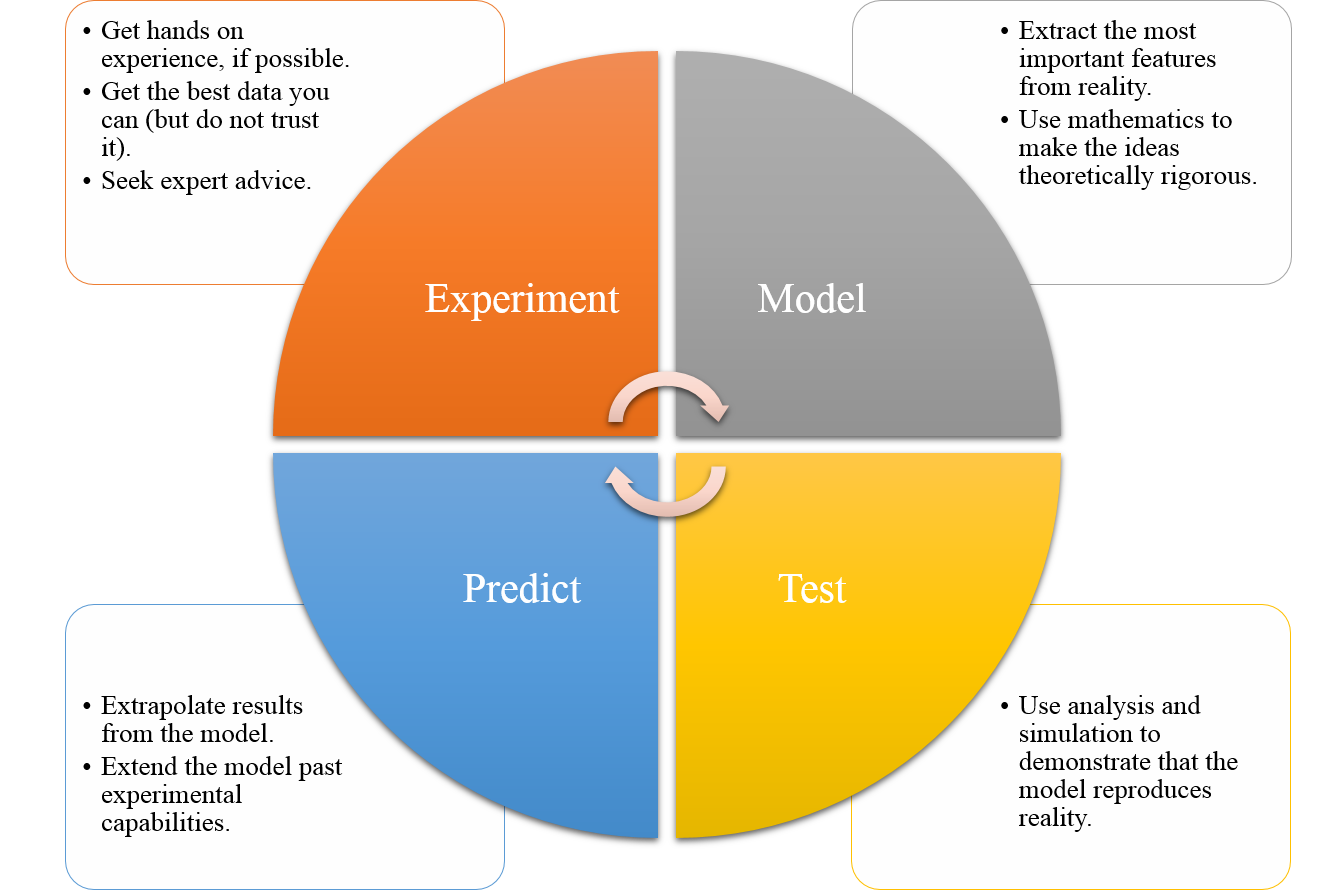
\includegraphics[width=\tp]{../Pictures/Modelling_loop.png}
\caption{\label{Modelling_loop}Diagram of the modelling cycle.}
\end{figure}

In this chapter we are going to review some of the methods that can be used to produce a mathematical interpretation of reality.

\section{Physical laws}
\begin{defin}
A \textbf{constitutive relation} (or `physical law') is a rule that the modeller adds to the system based on their experimental experience, which relates interacting components.
\end{defin}
Physics has many laws such as: conservation of energy, general relativity and the laws of thermodynamics. There is (as yet) no fundamental reason for these laws to hold. We just take them as laws because they fit the data that we observe.

Here are just a few examples of the laws that you might come across.
\begin{itemize}

\item \textbf{Newton's Law of Cooling.}

\textit{The rate of cooling of a body is proportional to the difference between the bodies temperature and the temperature of its environment.}

\COL{Let $T$ and $T_e$ be the temperatures of the object and the environment, respectively, then
\bb
\dot{T}=k(T_e-T),\label{Law_of_cooling}
\ee
where $k$ is defined to be the heat transfer coefficient.}
\begin{example}[frametitle=Cooling tea]\label{Cooling_tea}
Suppose I prepare two cups of tea at exactly the same time, so initially they both start at $100^o$C. I quickly add enough milk to cup 1 to cool it to $90^o$C. Ten minutes later I add milk to cup 2, which cools cup 2 by $10^o$C. Which cup is hotter at that point?
\COL{
The general solution to \eqn{Law_of_cooling} is
\bb
T(t)=T_e+\l T(0)-T_e\r e^{-kt},
\ee
where $T(0)$ is the initial temperature. For cup 1 we have
\bb
T_1(10)=T_{e}+\l 90-T_{e}\r e^{-k10}.
\ee
For cup 2 we have
\bb
T_2(10)=T_{e}+\l 100-T_{e}\r e^{-k10}-10.
\ee
Subtracting $T_1$ from $T_2$ gives
\bb
T_1(10)-T_2(10)=10\l 1- e^{-k10}\r>0.
\ee
Since $\exp(0)=1$ and $\exp(-kt)$ is a strictly monotonically decreasing function of time. Hence, cup 1 is hotter than cup 2 at time $t=10$ minutes. This means that the earlier you put your milk in the hotter your tea will stay!

Note that neither the ambient temperature, nor the heat transfer coefficient were needed.}
\end{example}

\item \textbf{Newton's Second Law of Motion}

\textit{The rate of change of momentum of a body is directly proportional to the force applied to the body.}

\COL{This is the standard $F=ma$ that everyone knows and loves (assuming that the mass remains that same throughout the interaction), where the acceleration, $a$, is the second derivative of the location with respect to time, $a=\ddot{x}$.}


\item \textbf{Newton's Law of Gravitation}\footnote{Newton devised the laws of optics, the laws of motion and invented calculus practically on a dare... then he turned 26. What have you done today? }

\textit{A particle attracts every other particle in the universe using a force that is directly proportional to the product of their masses and inversely proportional to the square of the distance between their centres.}

\COL{Suppose body $i$ has mass $m_i$ and is at position $\bm{r}_i=(x_i,y_i)$. Body $i$ is then separated from body $j$ by a distance $r_{ij}=\sqrt{\l x_i-x_j\r^2+\l y_i-y_j \r^2}=|\bm{r}_i-\bm{r}_j|$. Let $G$ be the universal gravitational constant then the force, $\bm{F}_{ij}$, acting on body $i$ from body $j$ is
\bb
\bm{F}_{ij}=-G\frac{m_im_j}{r^2_{ij}}\bm{\hat{r}}_{ji},
\ee
where 
\bb
\bm{\hat{r}}_{ji}=\frac{r_i-r_j}{|r_i-r_j|}
\ee
is the unit vector from body $j$ to body $i$.

Note that the force is vector valued quantity because it has a magnitude, but also a direction, as it acts in the direction of the line joining the bodies.}
\begin{figure}[!!!h!!!tb]
\centering
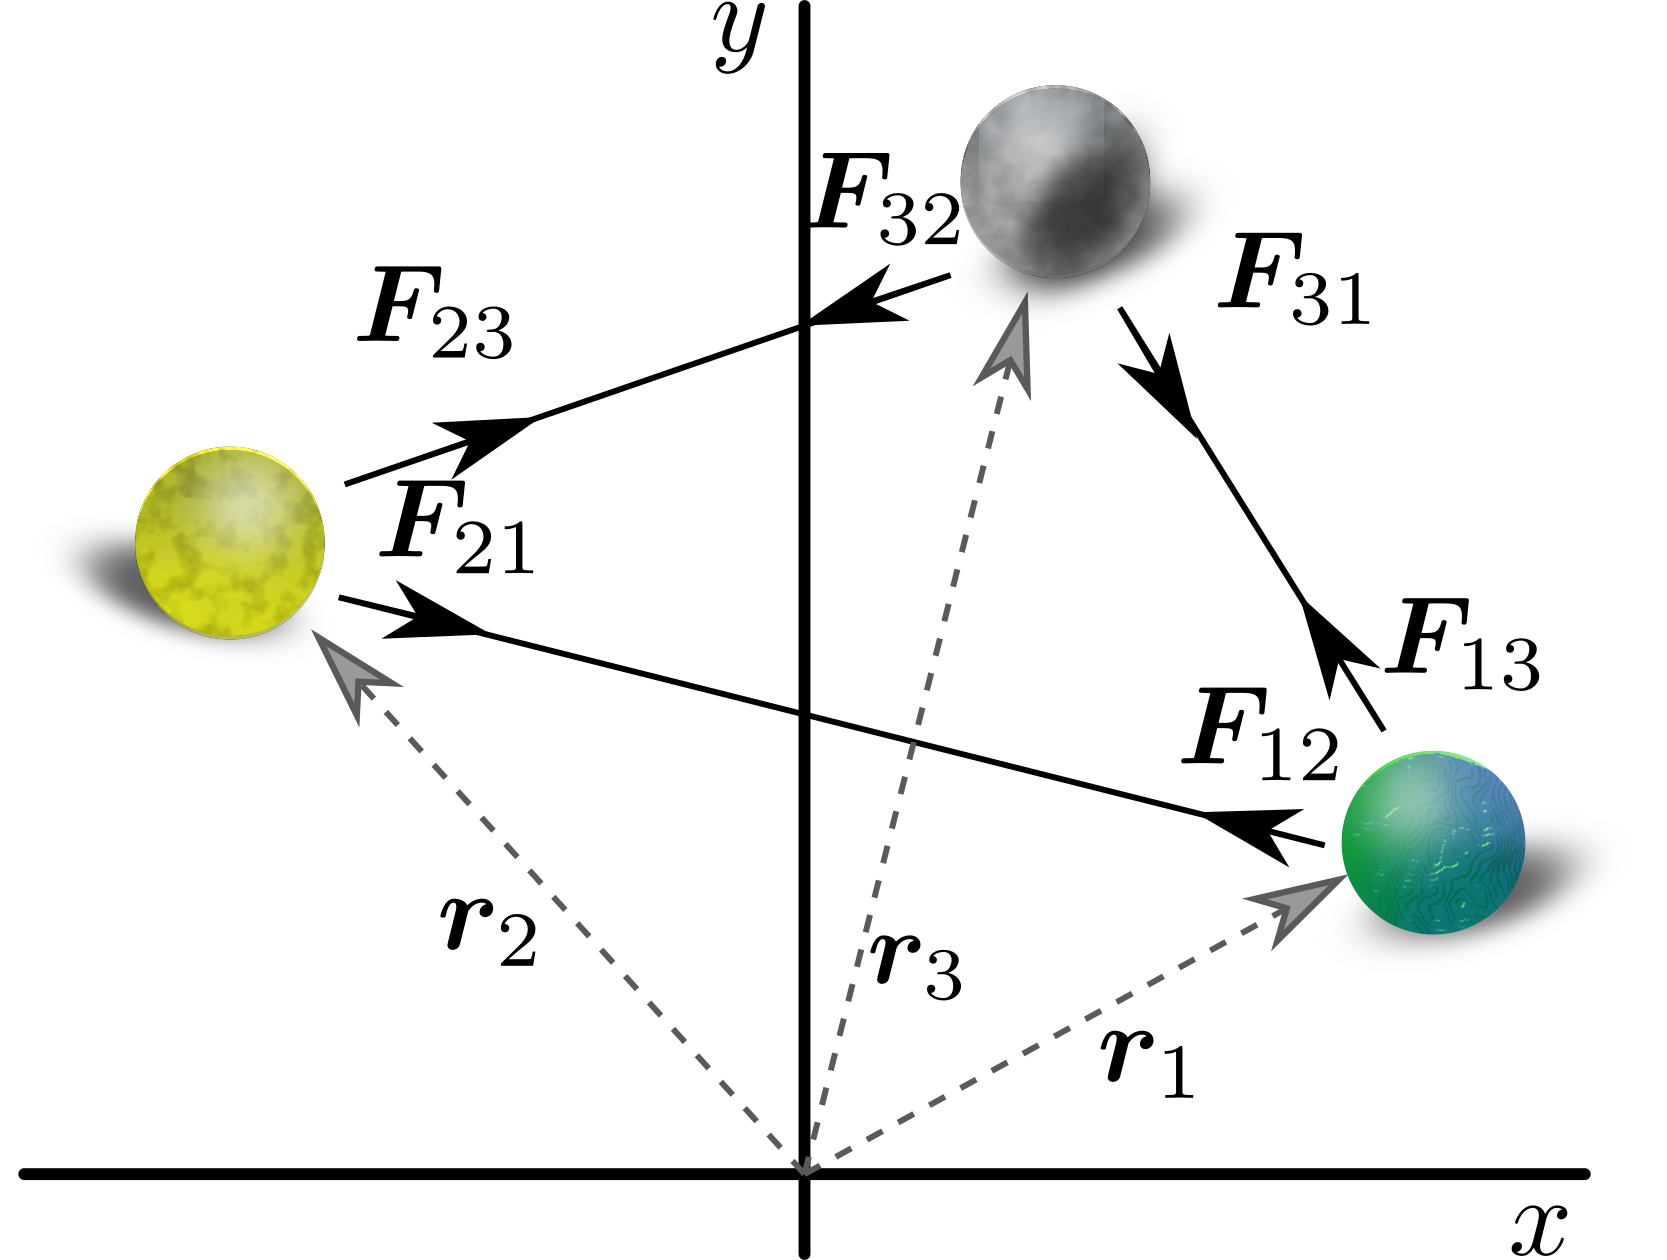
\includegraphics[width=\ttp]{../Pictures/Three_body_problem.png}
\caption{\label{Three_body}Schematic diagram of the three-body problem.}
\end{figure}


\begin{example}[frametitle=Three body problem]\label{Three_body_problem}
We can combine the Second Law of Motion and the Law of Gravitation in order to predict the position of planets interacting through their gravitational fields \see{Three_body}. Consider three planets with the same mass, $m$, and positions $\bm{r}_1(t)$, $\bm{r}_2(t)$ and $\bm{r}_3(t)$, respectively. Further, we note that since we are dealing with acceleration (a second order equation) we will need to specify two initial conditions, the position and velocity. Let the initial positions be $\bm{r}_i(0)=\bm{r}_{i0}$ and the initial velocities $\dot{\bm{r}}_i(0)=\bm{v}_{i0}$.\COL{ The governing equations are
\begin{align}
&m\ddot{\bm{r}}_1=-G\frac{m^2}{|\bm{r}_1-\bm{r}_2|^3}\l\bm{r}_1-\bm{r}_2\r-G\frac{m^2}{|\bm{r}_1-\bm{r}_3|^3}\l\bm{r}_1-\bm{r}_3\r,\label{g1}\\
&m\ddot{\bm{r}}_2=-G\frac{m^2}{|\bm{r}_2-\bm{r}_1|^3}\l\bm{r}_2-\bm{r}_1\r-G\frac{m^2}{|\bm{r}_2-\bm{r}_3|^3}\l\bm{r}_2-\bm{r}_3\r\label{g2},\\
&m\ddot{\bm{r}}_3=-G\frac{m^2}{|\bm{r}_3-\bm{r}_1|^3}\l\bm{r}_3-\bm{r}_1\r-G\frac{m^2}{|\bm{r}_3-\bm{r}_2|^3}\l\bm{r}_3-\bm{r}_2\r\label{g3}.
\end{align}
where we remember that this is a vector equation, $\bm{r}_i=(x_i,y_i)$, so there are actually six, second order ODEs here, rather than three.}

The three body problem illustrates chaotic behaviour, in the sense that the outcome is extremely sensitive to the initial conditions. This can be seen in the simulations of \fig{Three_body_sim}.

Simulation tip:
\begin{itemize}
\item when solving \eqnto{g1}{g3} numerically we could separate each equation into its Cartesian components and reduce the second order equation to two first order equations. Namely, we would introduce $(v_{ix},v_{iy})=(\dot{x}_i,\dot{y}_i)$. Thus, we would have a system of twelve ODEs to solve, with variables
\bb
(x_1,y_1,v_{1x},v_{1y},x_2,y_2,v_{2x},v_{2y},x_3,y_3,v_{3x},v_{3y}).
\ee
However, since $x_i$ and $y_i$ are perpendicular Cartesian coordinates it turns out to be a good idea to use complex numbers. Specifically, instead of writing two ODEs for each of $x_i$ and $y_i$ we can simply solve one ODE in terms of the complex quantity $\bm{r}_i=x_i+Iy_i$, which can be handled by numerical solvers. Thus, we simplify the numerical solution from twelve to six equations.
\end{itemize}
\end{example}
\begin{figure}[!!!h!!!tb]
\centering
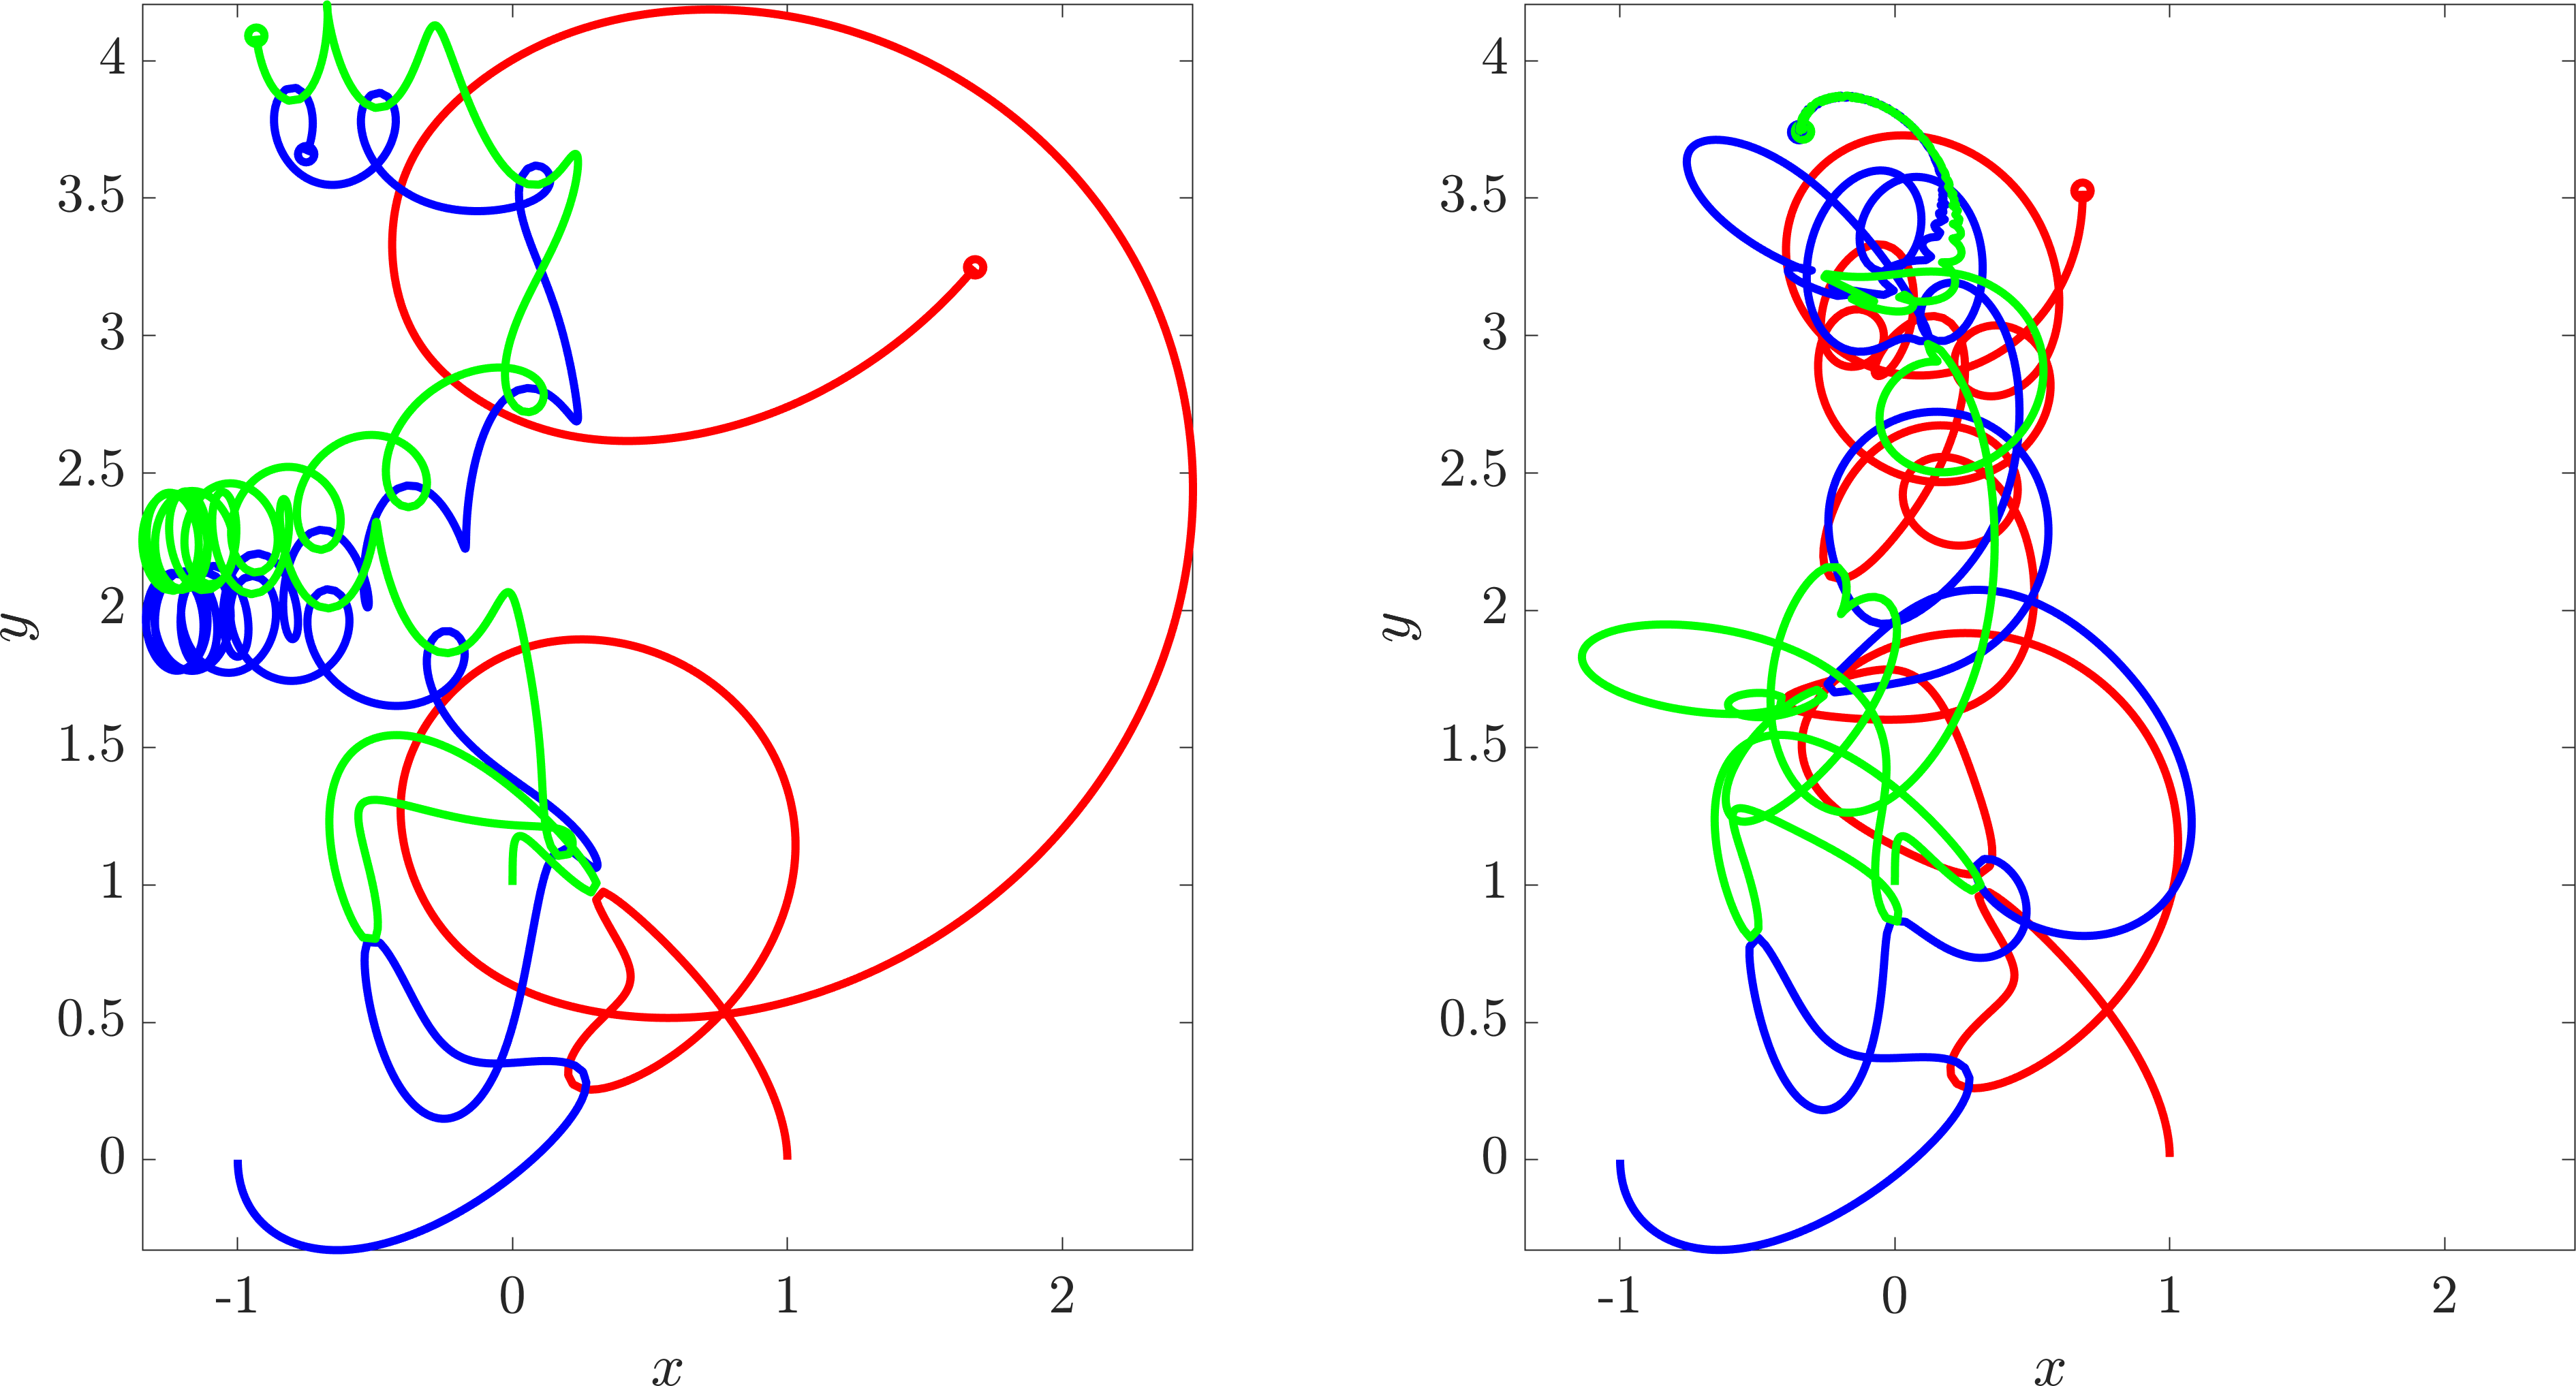
\includegraphics[width=\tp]{../Pictures/Three_body_sim.png}
\caption{\label{Three_body_sim}Two simulations of the three body problem. The green and red trajectories are identically initiated. The blue trajectory is initiated at $(-1,0.01)$ in the left figure and at $(-1,0)$ in the right figure.}
\end{figure}
\item \textbf{Hooke's law}

\textit{The force, $F$, needed to extend or compress a spring by some distance, $x$, scales linearly with respect to that distance,}
\COL{
\bb
F=kx.
\ee

The constant of proportionality, $k$, defined by this law is known as the spring constant and is measured in units of Force per distance, \eg N/m.

Depending on the material Hooke's law only holds true for small extensions and compressions. For example, this law suggests that given enough force a spring can pass through itself. Further, biological materials may not follow the law because they break if stretched too far (\eg bone), or they may grow, or permanently deform\footnote{Consider, for example, the ear. Small earrings to not stretch the skin very much and, thus, once the earring is removed the skin can heal. Alternatively, people who use large gauge earrings stretch their ear holes beyond the elastic limit of the skin so that they have a permanent hole. }, thus, reducing the force needed to give the same extension (\eg skin).
}

\end{itemize}
\subsubsection{Pendulums}\label{Pendulums_section}
In this section we take an extended look at pendulums depending on Hooke's law and simple Newtonian mechanics. Specifically, we consider a spring, oscillating up and down, and a bob, oscillating side to side \see{Pendulums}.
\begin{figure}[!!!h!!!tb]
\centering
\subfigure[\label{Spring}]{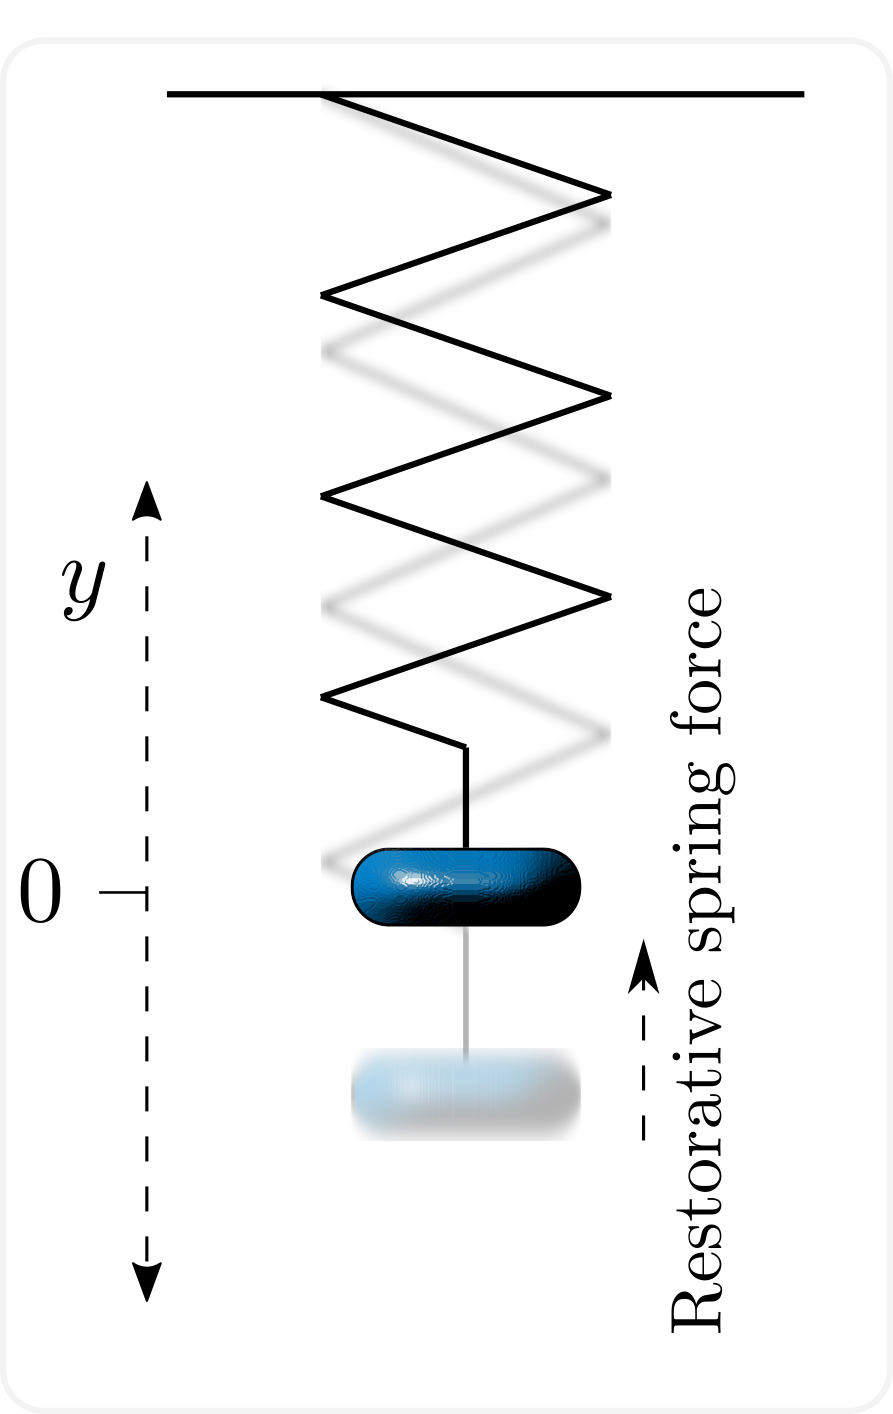
\includegraphics[width=\ttp]{../Pictures/Spring.png}}
\subfigure[\label{Bob}]{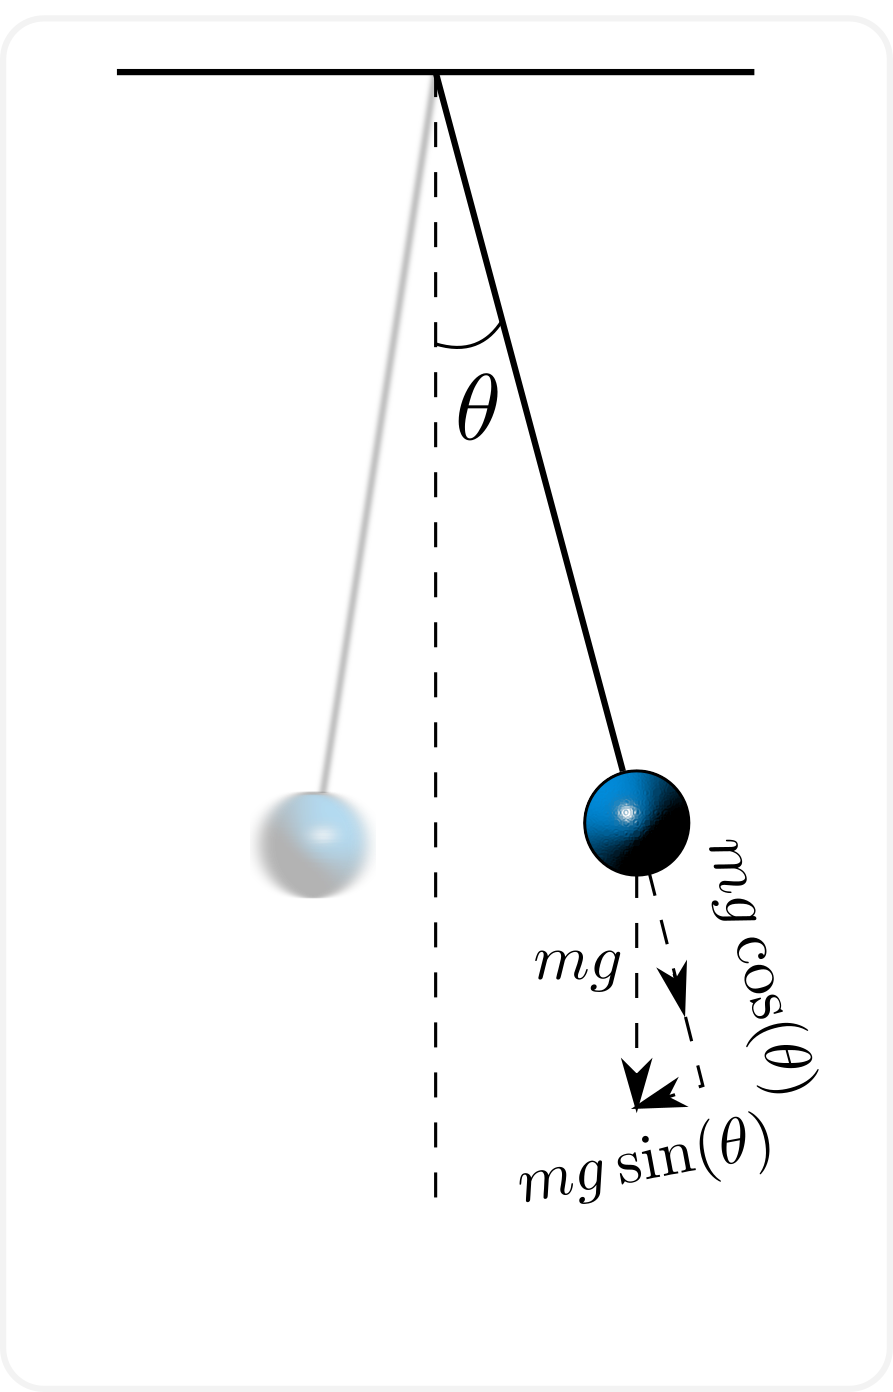
\includegraphics[width=\ttp]{../Pictures/Pendulum.png}}
\caption{Two types of pendulums: (a) an oscillating spring. (b) a weight on a string.\label{Pendulums}}
\end{figure}

\COL{Assuming that the spring conforms to Hooke's Law and applying Newton's Second Law of motion the equation of motion for the spring is
\bb
m\ddot{y}=-ky,\label{Spring_eqn}
\ee
where $y$ is the vertical displacement of the spring, $m$ is the mass attached to the spring and $k$ is the spring constant. The negative sign shows that the force is always directed to the resting position of the spring (here, taken to be the origin). If the negative sign was not there then we would be saying that the pendulums position would grow exponentially with an applied force, which is not very realistic.

The pendulum bob is slightly more complicated as we have to account for two-dimensional motion. Complicating the matter further is that the pendulum weight is confined to move on the arc of a circle, meaning that problem is easier to solve in polar coordinates.

To derive the equations of motion we split the component of force acting on the pendulum into components acting along the radial and angular directions of the system, as shown in \fig{Bob}. Critically, we only need to consider the angular acceleration, which can be derived to be $r\ddot{\theta}$. The derivation will be seen on problem sheet two. Using Newton's Second Law again we derive that
\bb
mr\ddot{\theta}=-mg\sin(\theta).\label{Bob_eqn}
\ee
One interesting point we can immediately see from \eqn{Bob_eqn} is that the mass of the pendulum does not influence the solution of the equation, which can be compared with the dependence of \eqn{Spring_eqn} on the mass. 

Equation \ref{Bob_eqn} can be solved directly in terms of `elliptic integrals', but this accounts to little more than integrating the equation twice and leaving the equation written in integral form. More insight to the solution can be gained if the angle of oscillation is small. In this case we can linearise the right-hand side of \eqn{Bob_eqn} by using Taylor series about zero, \ie $\sin(\theta)\approx\theta$. Hence, \eqn{Bob_eqn} can be approximated by
\bb
r\ddot{\theta}=-g\theta\label{Bob_eqn_approx},
\ee
which can be seen to be analogous to \eqn{Spring_eqn}.

If the different pendulums are displaced and released from rest then the amount of error introduced into the equation is determined by the initial displacement. \fig{Different_ICs} compares\footnote{Comparing $y$ and $\theta$ is a little dodgy as $y$ is a dimensional length and the $\theta$ is dimensionless, as we work in radians. However, if this bothers you we can fix this is in either of two ways. Either, we consider $y$ normalised by its natural length (taken here to be of unit length, regardless of the dimensions involved), or, we can consider \fig{Different_ICs} comparing \eqn{Bob_eqn} and its approximation in \eqn{Bob_eqn_approx}.} \eqns{Spring_eqn}{Bob_eqn} with different initial conditions. Thus, we see that increasing the initial amplitude of the bob pendulum causes the wave length of the oscillation to increase, or frequency of oscillation to decrease.}
\begin{figure}[!!!h!!!tb]
\centering
\subfigure[\label{IC_0.1}]{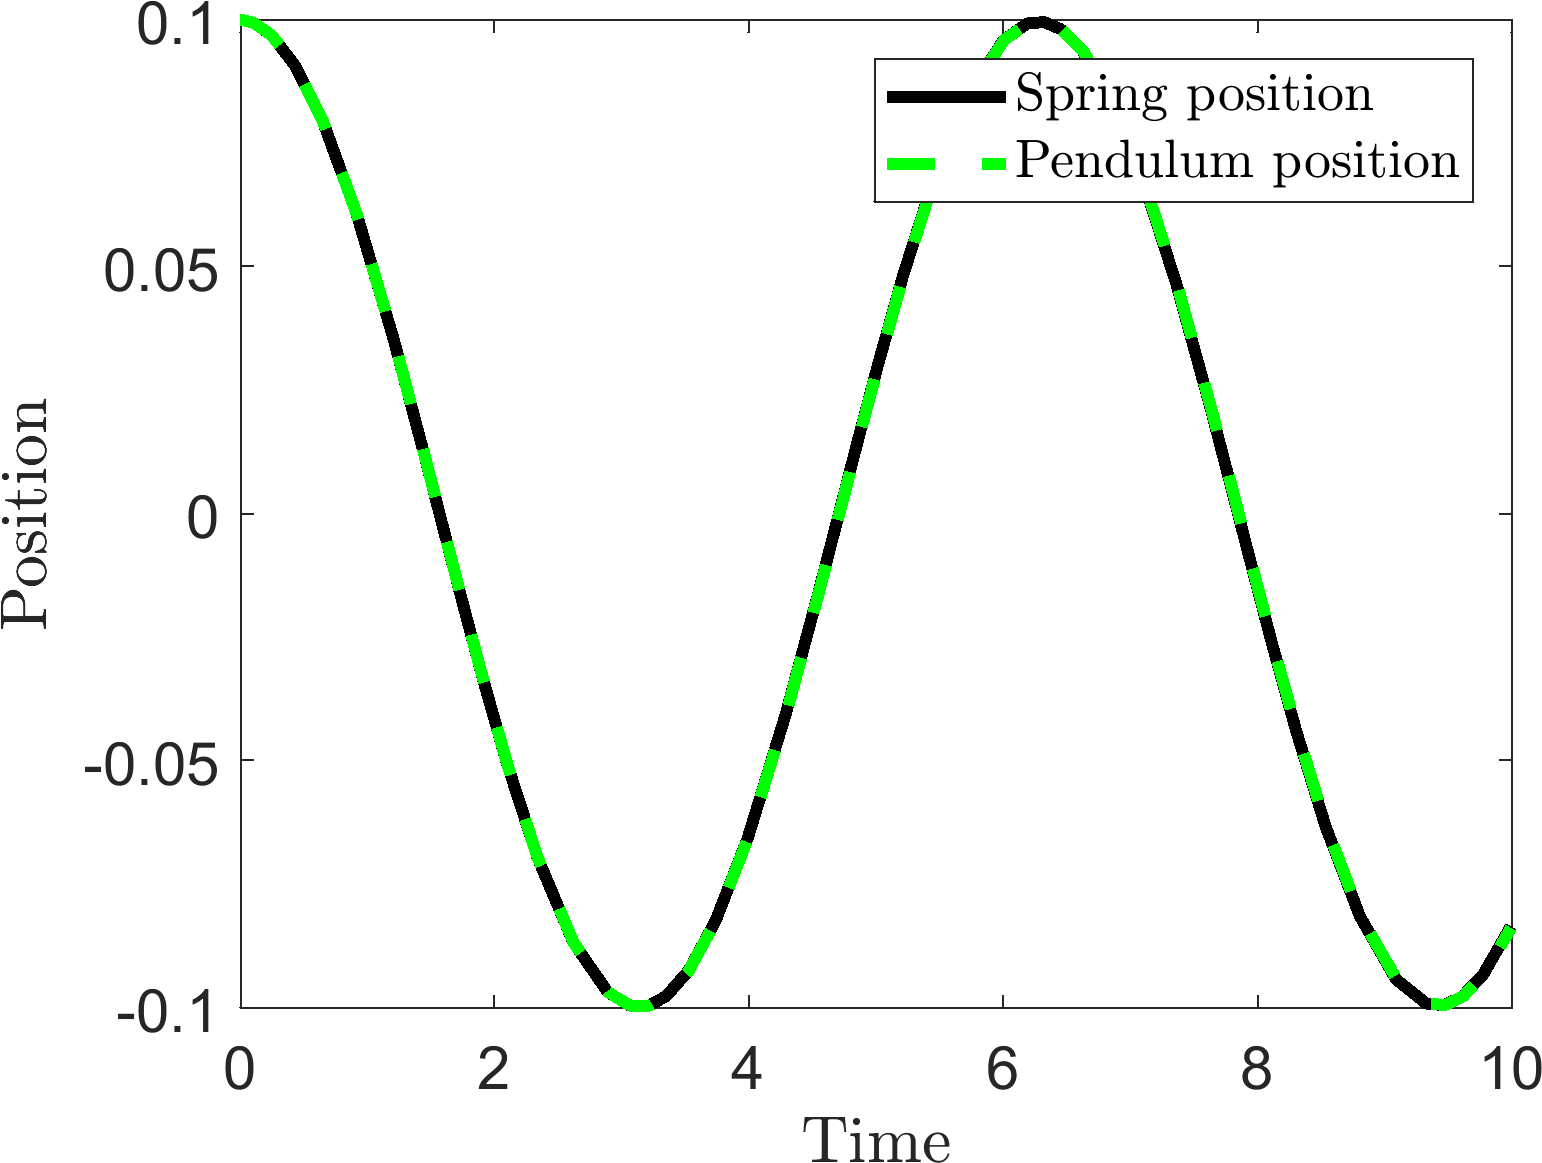
\includegraphics[width=\ttp]{../Pictures/Comparing_pendulums_IC_1.png}}
\subfigure[\label{IC_1}]{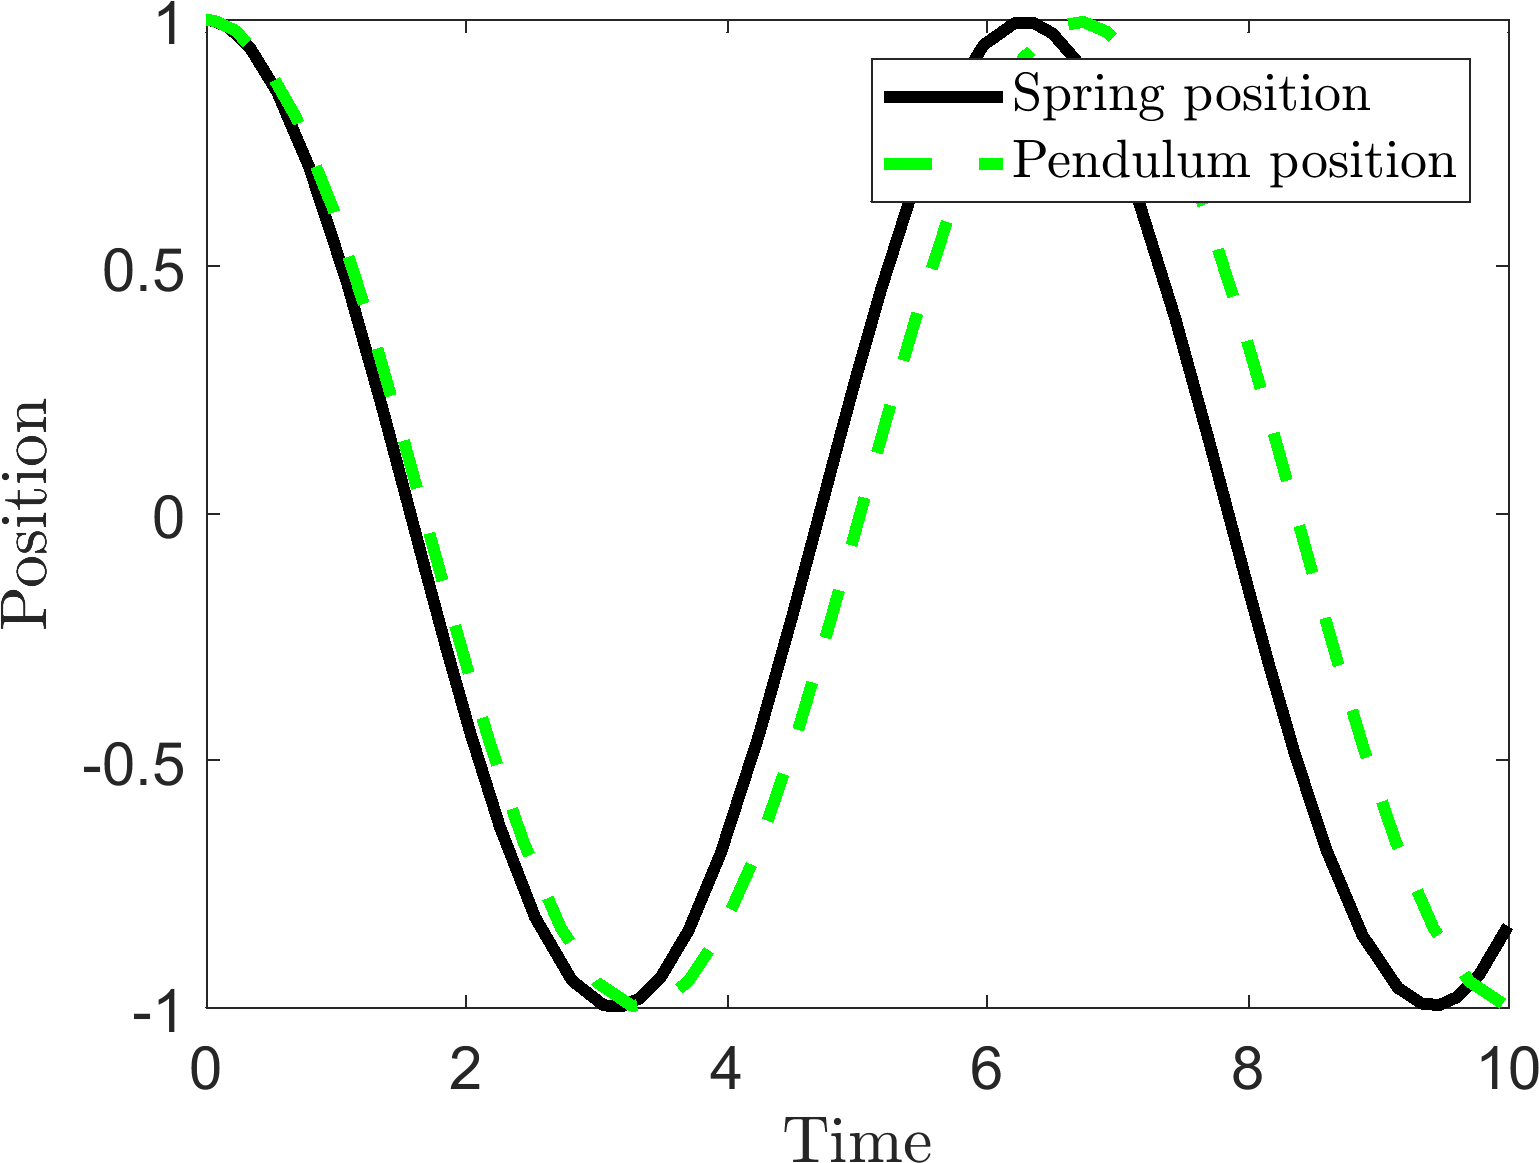
\includegraphics[width=\ttp]{../Pictures/Comparing_pendulums_IC_10.png}}
\caption{\label{Different_ICs}Comparing \eqns{Spring_eqn}{Bob_eqn} with initial conditions (a) $y=0.1=\theta$ and (b) $y=1=\theta$. Parameter values $r=g=k=m=1$.}
\end{figure}

\begin{defin}
Any system defined by an equation of the form
\bb
\ddot{u}=-k^2u.\label{SHM}
\ee
is said to under go \textbf{simple harmonic motion}.
\end{defin}
Equation \ref{SHM} can be solved to produce the solution
\bb
u=A\cos(kt)+B\sin(kt),
\ee
where $A$ and $B$ are specified through the initial conditions.

%\subsection{Euler-Bernoulli beam}
\section{Law of Mass Action}
All of the above physical laws are very specific in their application. In this section we will learn about a much more general technique that will allow us to build an ODE system out of multiple interacting populations. These populations could represent chemical compounds, humans, cells or animals as well as different states within a population \ie infected humans and susceptible humans. The law presented in this section is applied whenever the populations of the system are able to: (i) change identities; (ii) create more population members; or (iii) cause populations to decay. Specific examples of each of these interactions are, respectively: (i) susceptible humans becoming infected through interactions with a diseased person; (ii) animals giving birth; (iii) predators eating prey. Note that a change-of-identity interaction can itself be thought as a combination of creation and degradation operations. For example, in the above case of infection a member of the susceptible human population is removed from the system, whilst an infected human is added to the system. Thus, all interactions can be made through combining creation and degradation operations.

We use chemical reaction notation to specify the outcomes of population interactions. Consider a system composed of $n$ different interacting populations $(u_1,\dots,u_n)$. We assume that all interactions between the population elements lead to the creation, or destruction, of one (or more) of the $n$ populations. 
\begin{defin}
A \textbf{rate equation} specifies that an interaction involves $a_1$ members of population $u_1$, $a_2$ members of population $u_2$, etc. and produces $b_1$ members of population $u_1$, $b_2$ members of population $u_2$, etc. The equation is written as
\bb
a_1u_1+a_2u_2+\dots+a_nu_n \stackrel{r}{\rightarrow} b_1u_1+b_2u_2+\dots+b_nu_n,
\ee
where $r>0$ is the \textbf{reaction rate}.
\end{defin}
Note that some of the $a_i$ and $b_i$ values can be zero.

\begin{example}[frametitle=Reaction equation examples]\label{Reaction equation examples}
\begin{itemize}
\item \textbf{Birth}

Two agents of population $u$ come together to produce a third,
\COL{\bb
2u\stackrel{r}{\rightarrow}3u.
\ee}
\item \textbf{Death}

An agent of population $u$ dies (or is destroyed) due to natural causes,
\COL{
\bb
u\stackrel{r}{\rightarrow}\slashed{0}.
\ee}

\item \textbf{Predation}

A predator population, $v$, converts energy from eating prey, $u$, into offspring,
\COL{
\bb
u+v\stackrel{r}{\rightarrow}2v.
\ee}

\item \textbf{Infection}

Consider a population of infected people, $I$, who are able to infect a susceptible population, $S$. Further, over time, the infected people recover and become susceptible again,
\COL{\begin{align}
I+S&\stackrel{r_1}{\rightarrow}2I,\\
I&\stackrel{r_2}{\rightarrow}S.
\end{align}}
\end{itemize}
\end{example}

Rate equations provide a rigorous way of defining all of the interactions a system is assumed to undergo. However, we still require a method of converting the rate equation into an ODE. This is the power of the Law of Mass Action.
\begin{defin}
The \textbf{Law of Mass Action} states that production rate of a reaction is directly proportional to the product of the input population sizes. Specifically, if 
\bb
a_1u_1+a_2u_2+\dots+a_nu_n \stackrel{r}{\rightarrow} b_1u_1+b_2u_2+\dots+b_nu_n \nonumber
\ee
is the reaction of interest then the production rate is proportional to
\bb
ru_1^{a_1}u_2^{a_2}\dots u_n^{a_n}
\ee
and the accompanying ODEs are
\begin{align}
&\dot{u}_1=(b_1-a_1)ru_1^{a_1}u_2^{a_2}\dots u_n^{a_n},\\
&\dot{u}_2=(b_2-a_2)ru_1^{a_1}u_2^{a_2}\dots u_n^{a_n},\\
&\vdots\\
&\dot{u}_n=(b_n-a_n)ru_1^{a_1}u_2^{a_2}\dots u_n^{a_n}.
\end{align}
\end{defin}
Note that in converting from reaction equation to the ODE of $u_i$ we to account for the stoichiometry, \ie $(a_i-b_i)$. Further, when multiple reactions are considered, the terms arising from the Law of Mass Action are simply added together as independent terms.

\begin{example}[frametitle=Law of Mass Action examples]\label{Law of Mass Action examples}
\begin{itemize}
\item \textbf{Birth}
\COL{\begin{align}
2u&\stackrel{r}{\rightarrow}3u,\nonumber\\
\implies &\dot{u}=ru^2.
\end{align}}
\item \textbf{Death}
\COL{\begin{align}
u&\stackrel{r}{\rightarrow}\slashed{0},\nonumber\\
\implies &\dot{u}=-ru.
\end{align}}

\item \textbf{Predation}
\COL{\begin{align}
u+v&\stackrel{r}{\rightarrow}2v,\nonumber\\
\implies &\dot{u}=-ruv,\\
&\dot{v}=ruv.
\end{align}}

\item \textbf{Infection}
\COL{\begin{align}
I+S&\stackrel{r_1}{\rightarrow}2I,\quad I\stackrel{r_2}{\rightarrow}S,\nonumber\\
\implies &\dot{S}=-r_1IS+r_2I,\\
&\dot{I}=r_1IS-r_2I.
\end{align}}
\end{itemize}
\end{example}



\begin{example}[frametitle=Zombies]\label{Zombies}
Humans, $H$, and zombies, $Z$, interact through the following three interactions \see{Zombie_picture}:
\begin{enumerate}
\item humans kill zombies at a rate $a$;
\item zombies kill humans at a rate $b$;
\item zombies infect humans at a rate $c$.
\end{enumerate}
The reaction equations for this system are,
\COL{\begin{align}
&H+Z\stackrel{a}{\rightarrow}H;\\
&H+Z\stackrel{b}{\rightarrow}Z;\\
&H+Z\stackrel{c}{\rightarrow}2Z.
\end{align}
}\COL{The ODE form of the system is
\begin{align}
&\dot{H}=-bHZ-cHZ=-\alpha HZ\\
&\dot{Z}=-aHZ+cHZ=\beta HZ.
\end{align}
Since $\alpha=b+c>0$ the population of $H$ is always decreasing. However, $\beta=c-a$, which could be either positive or negative. Critically, if $\beta>0\implies c>a$ then the zombie population will grow. Alternatively, if $\beta<0 \implies c<a$ then  the zombie population decreases. Thus, the survival of the human race all depends on the sign of $c-a$, which, explicitly, is the `net rate increase of zombies', \ie zombie production minus zombie destruction.}
\end{example}
\begin{figure}[!!!h!!!tb]
\centering
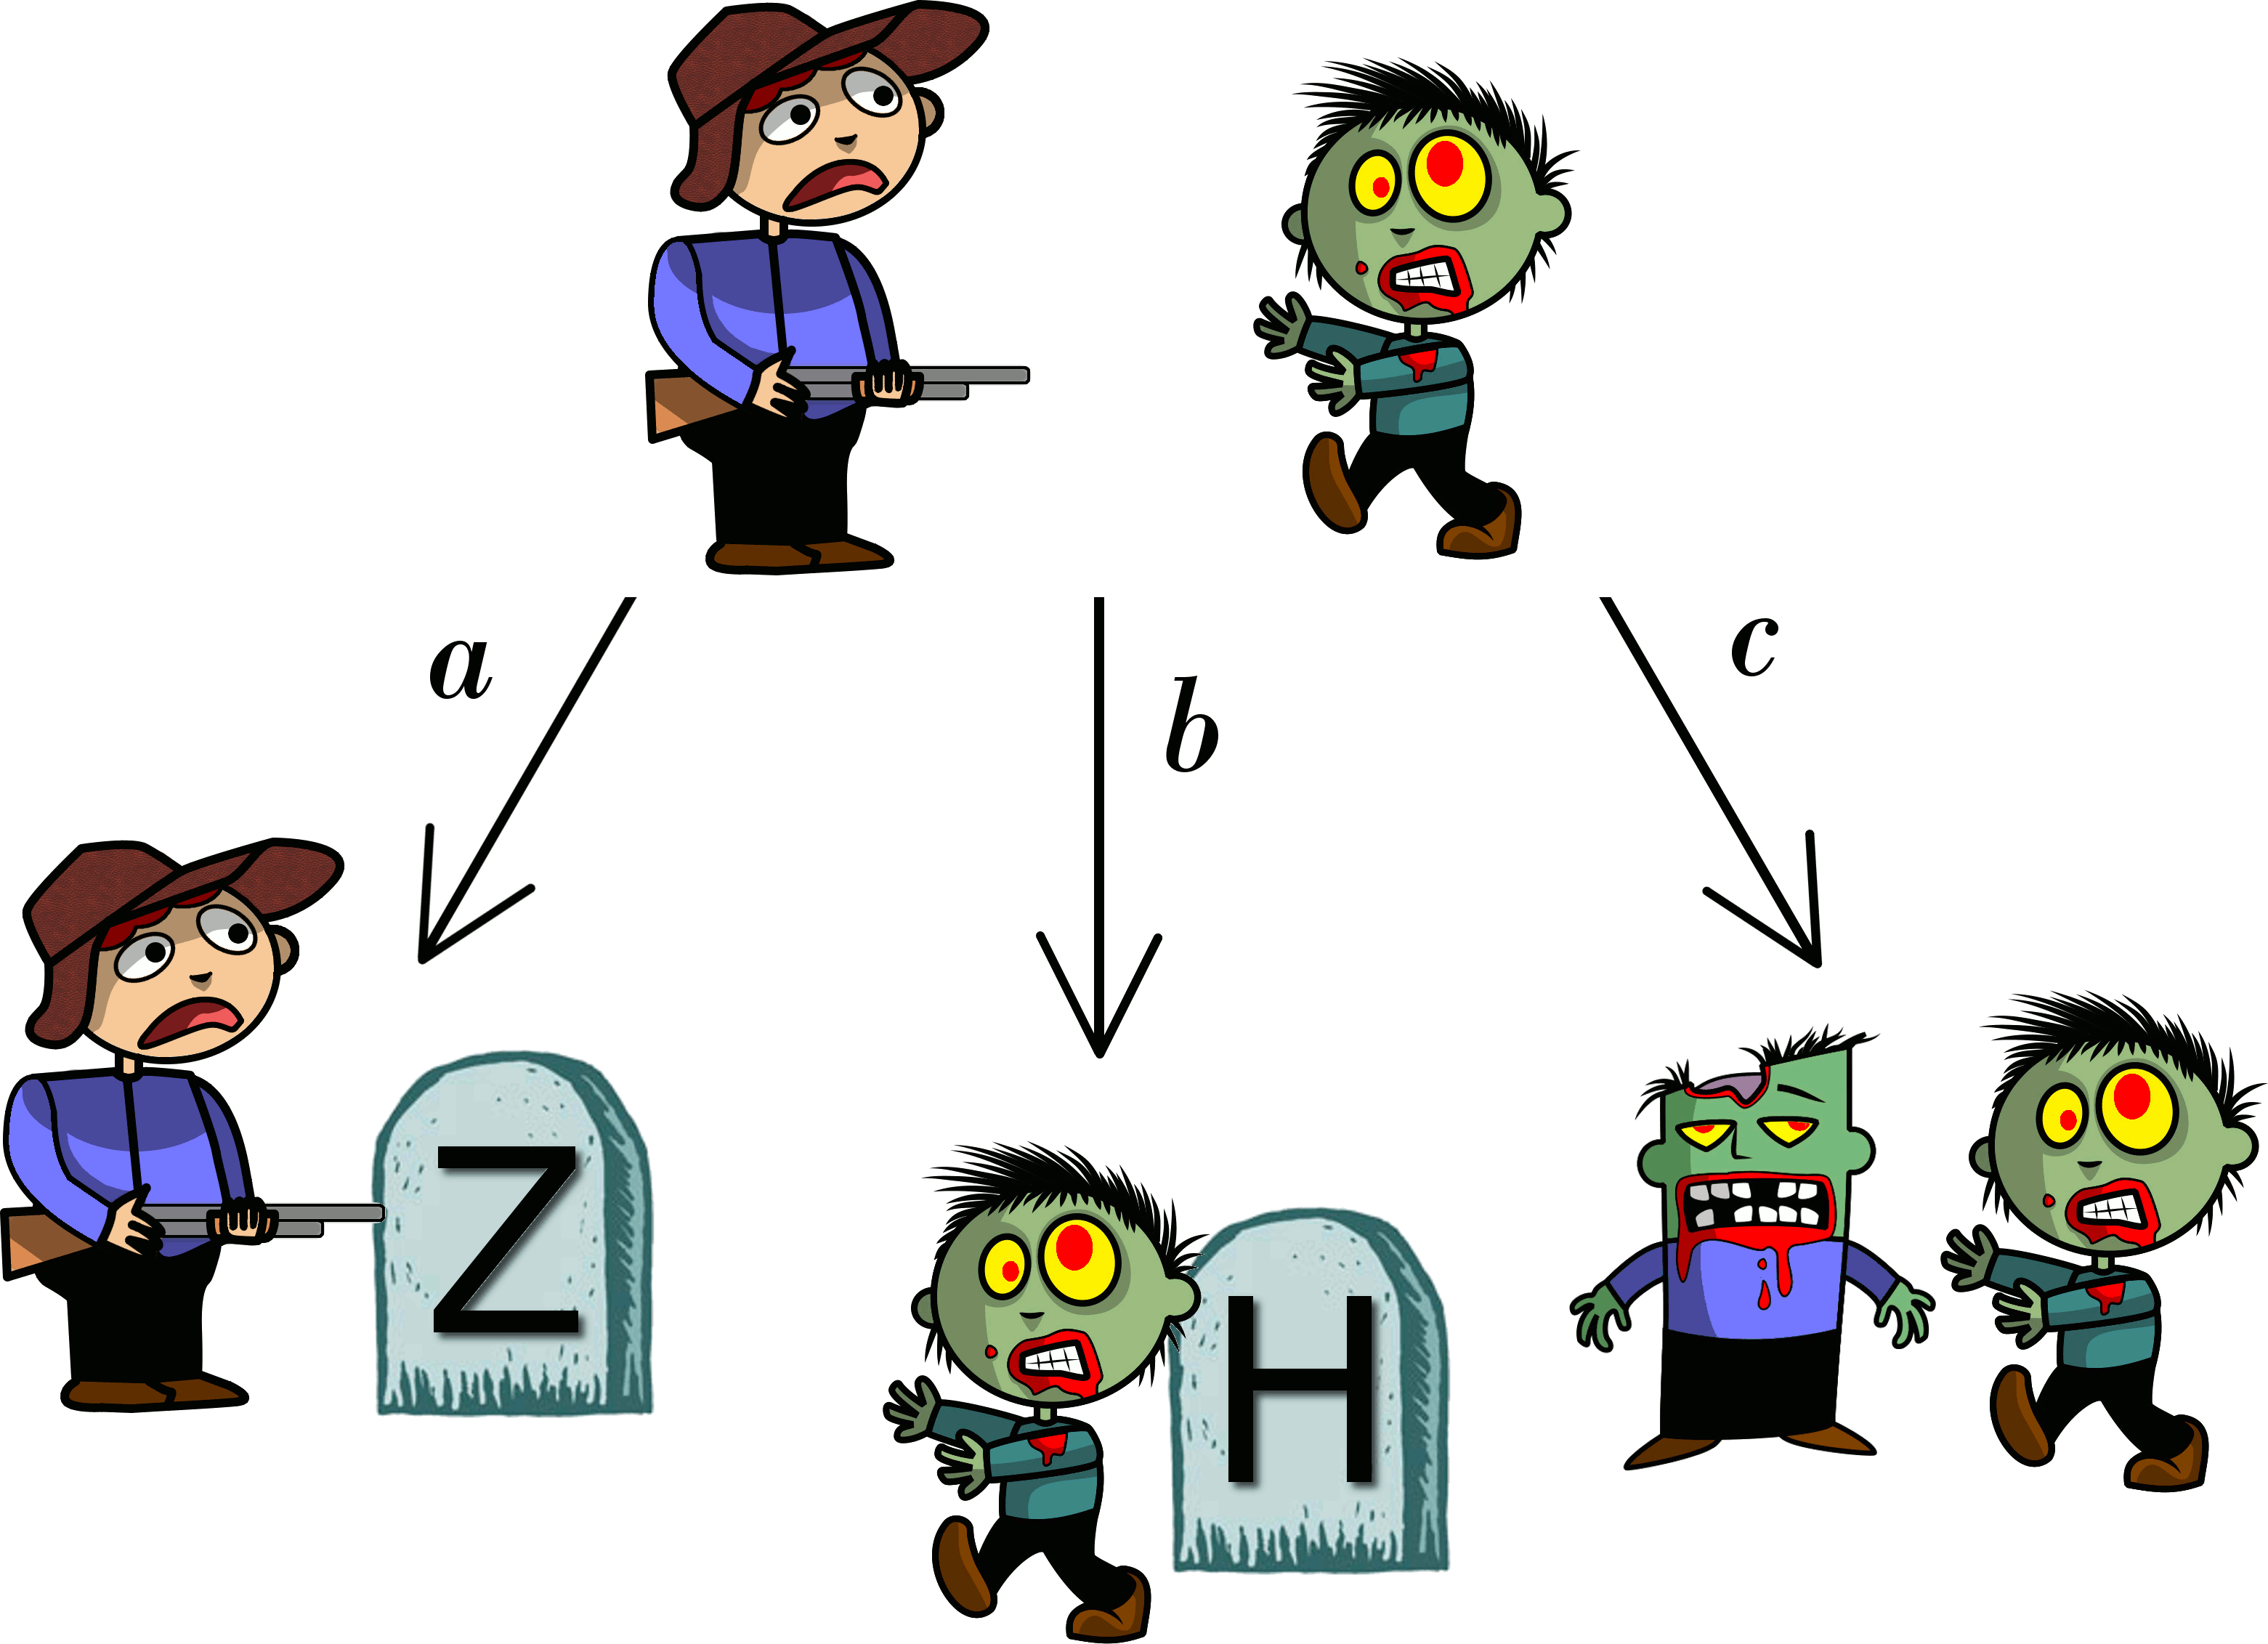
\includegraphics[width=\tp]{../Pictures/Zombies.png}
\caption{\label{Zombie_picture} Possible outcomes of human-zombie interactions.}
\end{figure}

\section{Check list}
By the end of this chapter you should be able to:
\begin{todolist}
\item define all of the constitutive laws;
\item solve problems involving Newton's laws, Hooke's law and simple harmonic motion;
\item convert a system of population interactions into reaction equations;
\item convert reaction equations into ODEs using the Law of Mass Action.
\end{todolist}




